%% LyX 2.2.3 created this file.  For more info, see http://www.lyx.org/.
%% Do not edit unless you really know what you are doing.
\documentclass[oneside,british,english]{extbook}
\usepackage[T1]{fontenc}
\usepackage[latin9]{inputenc}
\usepackage[a4paper]{geometry}
\geometry{verbose,tmargin=25mm,bmargin=25mm,lmargin=25mm,rmargin=25mm}
\setcounter{secnumdepth}{3}
\setcounter{tocdepth}{3}
\setlength{\parindent}{0bp}
\synctex=1
\usepackage{color}
\usepackage{babel}
\usepackage{float}
\usepackage{graphicx}
\usepackage{setspace}
\onehalfspacing
\usepackage[unicode=true,
 bookmarks=true,bookmarksnumbered=false,bookmarksopen=false,
 breaklinks=false,pdfborder={0 0 1},backref=false,colorlinks=true]
 {hyperref}
\hypersetup{
 pdfauthor={Juan Francisco Rasc�n}}

\makeatletter
%%%%%%%%%%%%%%%%%%%%%%%%%%%%%% User specified LaTeX commands.
\usepackage{amssymb}
\usepackage{color}
\usepackage{listings}
\definecolor{hellgelb}{rgb}{1,1,0.85}
\definecolor{colKeys}{rgb}{0,0,1}
\definecolor{colIdentifier}{rgb}{0,0,0}
\definecolor{colComments}{rgb}{1,0,0}
\definecolor{colString}{rgb}{0,0.5,0}
\lstset{
      language=Matlab,
      float=hbp,
      basicstyle=\footnotesize\ttfamily,
      identifierstyle=\color{colIdentifier},
      keywordstyle=\color{colKeys},
      stringstyle=\color{colString},
      commentstyle=\itshape\color{colComments},
      columns=fixed,
      tabsize=4,
      frame=single,
      framerule=1pt,
      extendedchars=true,
      showspaces=false,
      showstringspaces=false,
      numbers=left,
      numberstyle=\tiny\ttfamily,
      numbersep=1em,
      breaklines=true,
      breakindent=10pt,
      backgroundcolor=\color{hellgelb},
      breakautoindent=true,
      captionpos=t,
      xleftmargin=1em,
      xrightmargin=\fboxsep
}
\usepackage{lscape}
\usepackage{amsmath}
\usepackage{mathtools}
\usepackage{pifont}
\usepackage{color}
\usepackage{pdfpages}
\usepackage{accents}
\delimitershortfall=-1pt
\let\Right\right
\let\Left\left
\makeatletter
\def\right#1{\Right#1\@ifnextchar){\!\right}{}}
\def\left#1{\Left#1\@ifnextchar({\!\left}{}}
\makeatother

\setcounter{MaxMatrixCols}{20}

\makeatother

\begin{document}
\pagenumbering{gobble}

Why we achieve a pretty good path planning globally, I still have
to admit that, locally, the generated path is not drivable by a normal
car. So for example, let's consider a path like:

\begin{figure}[H]
\centering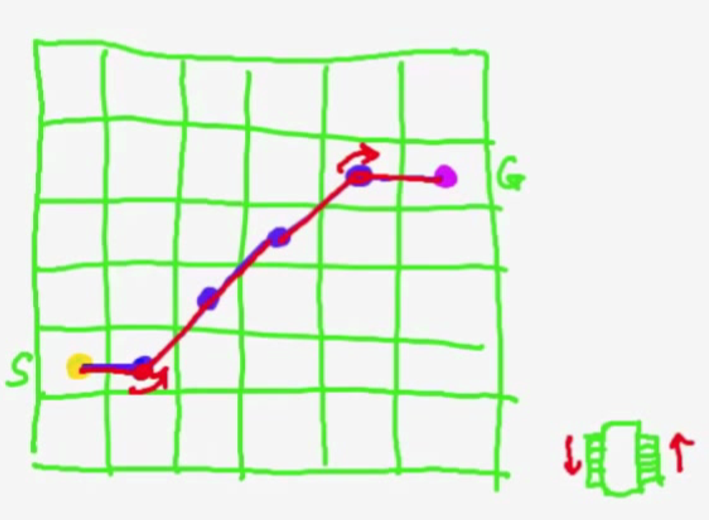
\includegraphics[scale=0.8]{../FIGURES/fig65}
\end{figure}

This path could be driven by a robot, for example the two-track robot
that we used on the SLAM lectures. This robot would drive straight
forward first, then it would move one track forward and the other
backwards, so it would turn in place, then it would drive straight
forward again, then it would turn in place again, then it would move
straight forward a bit more and finally it would have reached the
goal. However, a normal car has the constraints that it can only go
straight (either forward or backwards) or it can go along a circle,
where the radius of the circle is determined by the steering wheel.

\begin{figure}[H]
\centering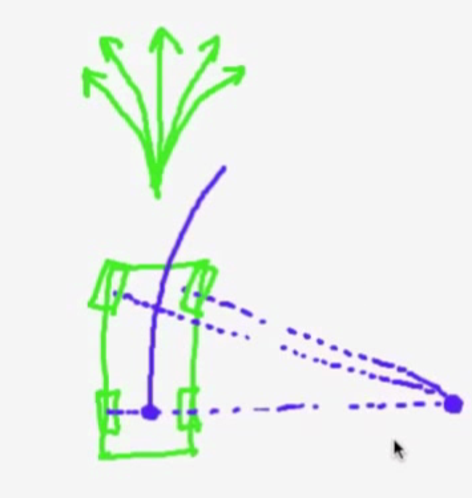
\includegraphics[scale=0.75]{../FIGURES/fig66}
\end{figure}

What we want now is to adapt the search for paths that can be driven
by a standard car. So, the we need to incorporate the car's constraints
to the algorithm. We will assume that our car can go either straight
or make a turn to the right or to the left, where those turns are
made of circular segments.

\begin{figure}[H]
\centering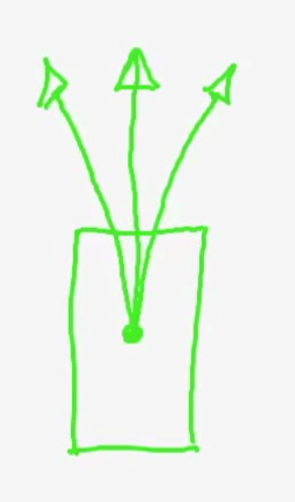
\includegraphics[scale=0.6]{../FIGURES/fig67}
\end{figure}

This model is more realistic than what we had earlier but you won't
find it on real roads. If you build a real road like that, consisting
of a straight line segment, then a circular segment, and then again
a straight line segment this would mean that a car coming from\texttt{A}
with certain speed would have to turn its steering wheel at infinite
speed at this point to make the right turn and then turn it back at
infinite speed at point B, which is unrealistic.

\begin{figure}[H]
\centering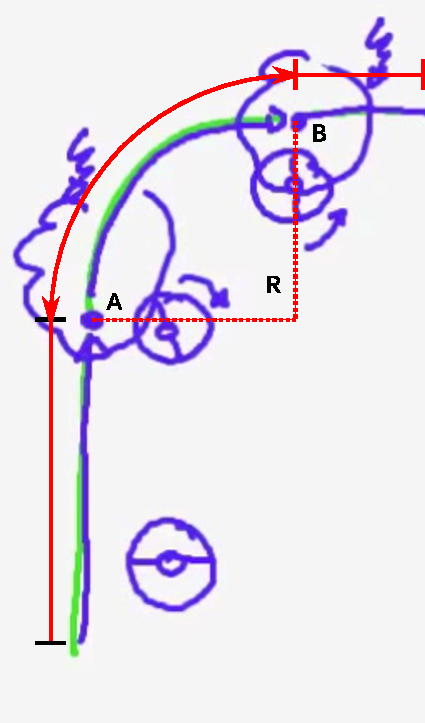
\includegraphics[scale=0.75]{../FIGURES/fig68}
\end{figure}

So, if you build streets in that way you will have a lot of accidents
at point A and B. However, this kind of navigation would be possible
at slow speeds for example on a parking lot, where the cars drive
slowly, then stand still, turn their wheels, and then go straight
into the parking lot.

\begin{figure}[H]
\centering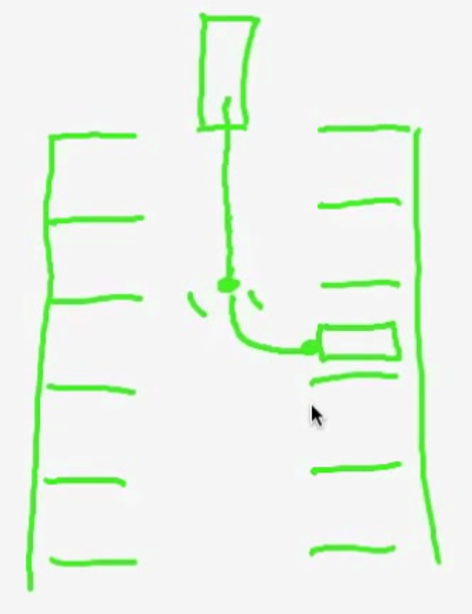
\includegraphics[scale=0.75]{../FIGURES/fig69}
\end{figure}

Imagine the car is at point A, in the next figure, and looking along
the x axis. Now, we do have coordinates$x$, and$y$, and a heading
angle,$\theta$, which together form the pose of the car,$\left(x, y,\theta\right)$.
Assume the point A is the starting point and we want to end at point
B, with a specific orientation. In this case, all the way from the
point A to the point B should be made up of straight line segments.

\begin{figure}[H]
\centering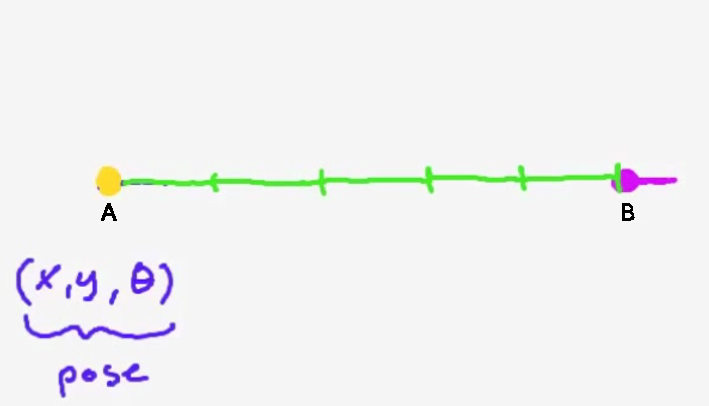
\includegraphics[scale=0.8]{../FIGURES/fig70}
\end{figure}

Now, imagine the situation of the next figure, where the car must
go from the point A to the point C.

\begin{figure}[H]
\centering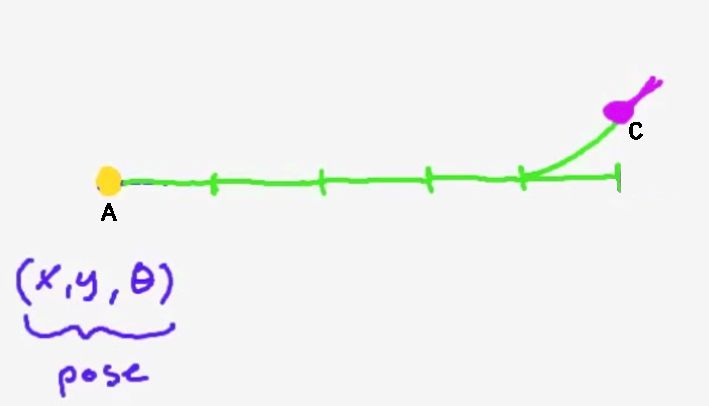
\includegraphics[scale=0.8]{../FIGURES/fig71}
\end{figure}

The car should describe the same trajectory but the last segment would
be replaced by a curved segment.

Right now, we will simplify the problem by considering three possible
curvatures only:
\begin{enumerate}
\item A curvature of zero,$C\, =\, 0$.
\item A positive constant curvature,$C\, >\, 0$.
\item A negative constant curvature,$C\, <\, 0$.
\end{enumerate}
So, the car can either go from the point A straight forward to the
point P1 or turn left to reach the point P2 or turn right to reach
the point P3. From the point P2 it can either go straight forward
to reach the point P5, or turn left to reach the point P4, or turn
right and reach the point P6. From the point P1 it can either go straight
forward to reach the point P7, or turn left to reach the point P8,
or turn right and reach the point P9 and so on and so forth.

\begin{figure}[H]
\centering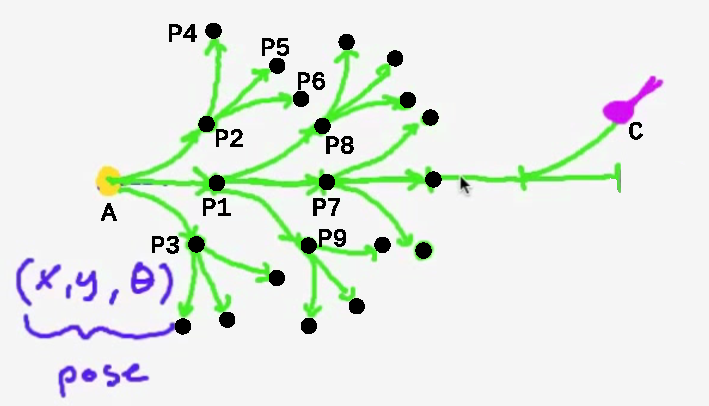
\includegraphics[scale=0.8]{../FIGURES/fig72}
\end{figure}

As you see, as before, the set of solutions expands a tree but now
this tree is in the kinematic state space of the car instead of being
in a raster as was the case in our previous implementations.

\begin{figure}[H]
\centering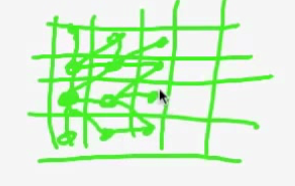
\includegraphics{../FIGURES/fig73}
\end{figure}
\begin{center}
\emph{(Remember, the car is moving in a world with obstacles, etc,
that is represented by a matrix, that has integral coordinates, i.e,
rows and columns. The real coordinates that the car reaches must be
converted into integral coordinates to access the corresponding cell
in the matrix and to observe if the robot can move there)}
\par\end{center}

Therefore, the algorithm will try to reach the goal pose, starting
from a specific starting pose, by exploring this tree. In order to
simplify matters, the standard length will be 5 units,$l\, =\, 5$,
and the allowed curvatures will be$C\,=\,\{ -1/10,\, 1/10\}$.

The algorithm starts marking the starting node (starting pose), node
A, as visited. Then it selects one of the \foreignlanguage{british}{neighbour}
nodes, in this case the node P1. Then, as in the A{*} implementation,
it computes the total cost for the node P1 as the distance from the
starting node (node A) to the node P1 plus the direct line distance
from P1 to the goal (node C) and inserts the node with its total cost
in the front list. Then the algorithm does the same operations with
the remaining \foreignlanguage{british}{neighbour} nodes, i.e, nodes
P2 and P3.

\begin{figure}[H]
\centering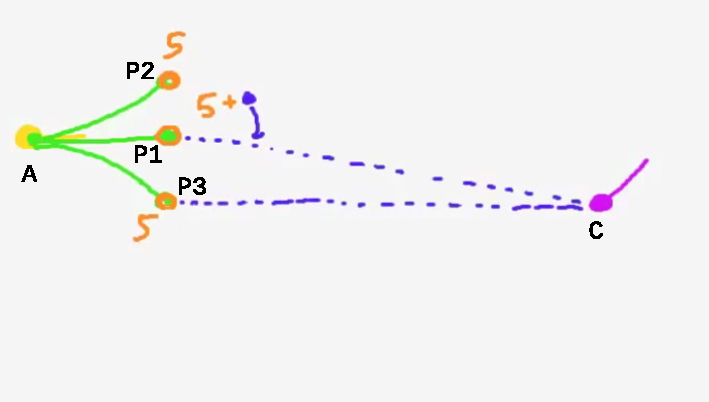
\includegraphics[scale=0.8]{../FIGURES/fig74}
\end{figure}

The driven distance in all those three cases is$l\, =\, 5$, therefore
the node P3 is the closest node to goal among the nodes P1, P2 and
P3. Then the algorithm selects the node with the smallest cost from
the front list and marks it as visited. This is the node P3. The algorithm
repeat the same procedure as the one it did for the node A. This is
what is called, expand the node. So, the algorithm expands the node
P3.

\begin{figure}[H]
\centering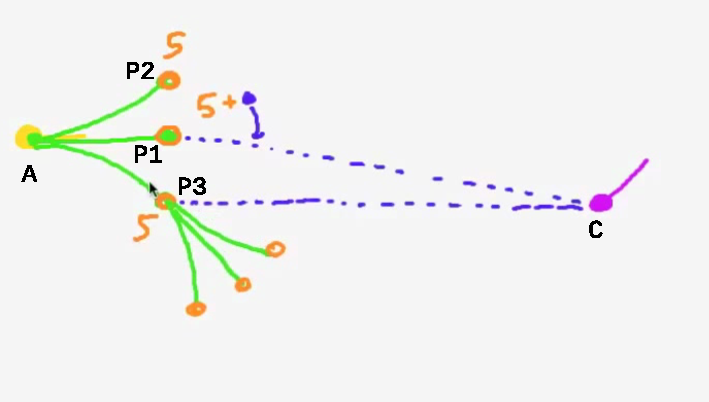
\includegraphics[scale=0.8]{../FIGURES/fig75}
\end{figure}

It is our hope that the algorithm will finally end up with a trajectory,
as the one shown in pink color in the next figure, that is able to
connect the starting node (node A) and the ending node (node C) combining
straight lines and circular segments.

\begin{figure}[H]
\centering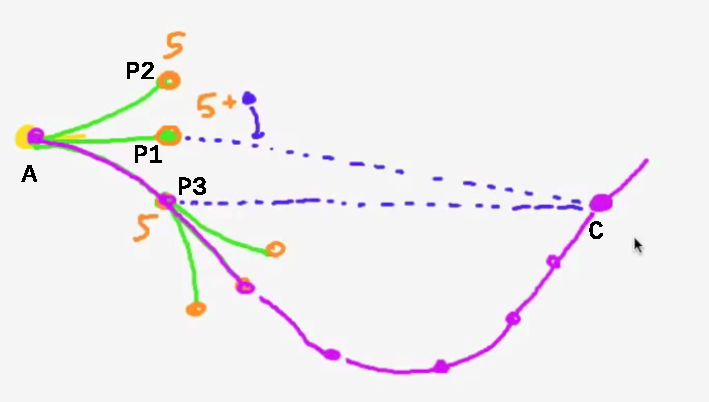
\includegraphics[scale=0.8]{../FIGURES/fig76}
\end{figure}

Again, what we explore here is the state space in terms of the controls
that the car can do, in this case, the steering angle, whereas earlier,
we have explored the space of possible positions in the plane without
worrying about if it is possible for a real vehicle to set its controls
in a way that it can actually follow this path.

\begin{figure}[H]
\centering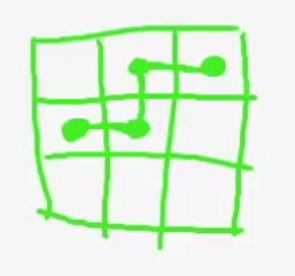
\includegraphics[scale=0.75]{../FIGURES/fig77}
\end{figure}

There's a small adjustment we have to make in the algorithm with regards
to the previous implementations. Since we allow only discrete lengths
and only discrete curvatures, in general, we will be unable to hit
the goal node, i.e, the goal pose or goal state, exactly. So, instead
of testing if we reach the goal state exactly, as we did earlier,
now we have to test if the current state is within a certain tolerance
in position and heading angle from the goal state, and if so we will
accepted this state.

\begin{figure}[H]
\centering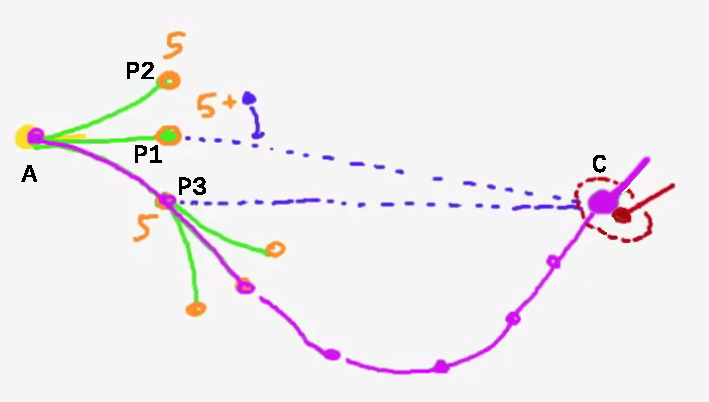
\includegraphics[scale=0.8]{../FIGURES/fig78}
\end{figure}

This is not very unrealistic because usually after having planned
that path we might still be able to fine-tune this trajectory, so
to use in detail a slightly different curvature to optimize the path
and end up in the correct position with the correct orientation.

\newpage

Let us compare the A{*} algorithm with the car path planning algorithm
that uses the kinematic state space of the vehicle. The A{*} algorithm
and the Dijkstra algorithm work with a raster of cells, so when they
visit a cell they can also explore all the \foreignlanguage{british}{neighbour}
cells and check what cells have to be put it into the front list.
The A{*} algorithm starts marking the starting node (node A in the
next figure) as visited. Then it selects one of the neighbour nodes,
in this case the node B. Then it computes the total cost for the node
B as the distance from the starting node (node A) to the node B, plus
the cost due to the potential field in the node B, if this issue is
considered, plus the direct line distance from B to the goal and then
it inserts the node B with its total cost in the front list. Then
the algorithm does the same operations with the remaining neighbour
nodes of node A.

\begin{figure}[H]
\centering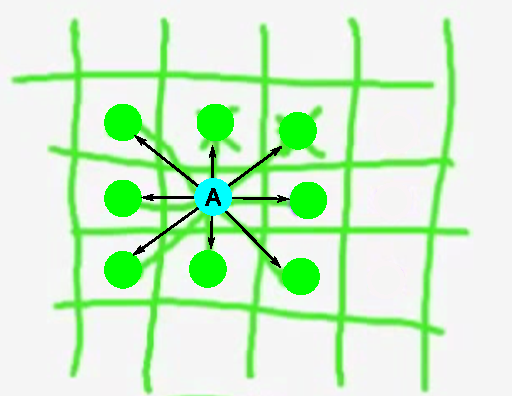
\includegraphics[scale=0.95]{../FIGURES/fig80}
\end{figure}

Let's consider that the node B is the node in the front list with
the smallest cost. Therefore, the algorithm pops the node B from the
front list and marks it as visited. Then, the algorithm checks the
neighbour nodes of node B except the node A which has already been
visited.

\begin{figure}[H]
\centering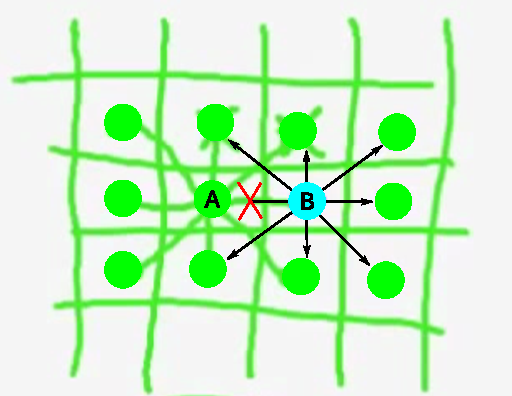
\includegraphics[scale=0.95]{../FIGURES/fig81}
\end{figure}

We see that this approach of discrete cells limits the amount of nodes
that are added to the front list while the algorithm procees in the
search of the optimal path between the starting node and the goal
node. Let's imagine that the Dijkstra algorithm runs for a while and
find the optimal path between the starting node (node A), and the
goal node (G), and this path is comprises by $d$ cells or nodes (not
necessarily in a straight line, although in this example they are
placed on a straight line).

\begin{figure}[H]
\centering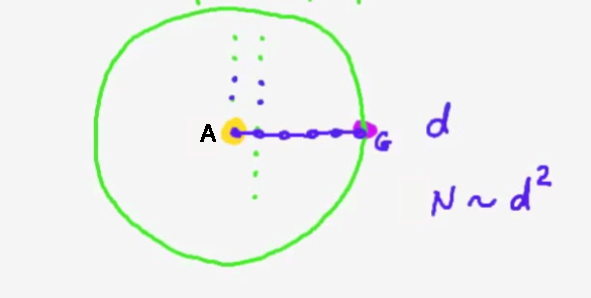
\includegraphics[scale=0.95]{../FIGURES/fig82}
\end{figure}

In the worst-case search (belonging to the Dijkstra algorithm, because
the A{*} algorithm is more goal-oriented) it will look like the circle
in the previous figure. All the nodes inside the circle will have
been visited. So, if the optimal path is comprises by $d$ steps,
then the number of nodes inside the circle is proportional to the
area of this circle, which is proportional to $d^2$.

\[
N \, \sim \, d^2
\]

That's bad, but it's not too bad and as we know we can help for a
better shape of the search space so that this number gets smaller,
although, of course, in general we will end up with $d^2$. A{*} algorithm
reduces the search space.

\begin{figure}[H]
\centering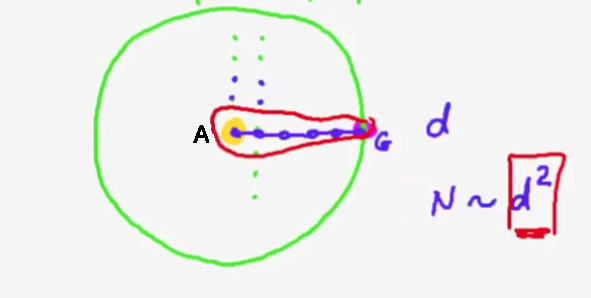
\includegraphics[scale=0.95]{../FIGURES/fig83}
\end{figure}

Now let's have a look at the new algorithm which operates in the kinematic
state space of the car. This new algorithm looks pretty much the same
as the A{*} algorithm, however, there is one aspect in where they
are different.

In the A{*} algorithm once the algorithm has visited a node it can
cross that node off, i.e, it marks the node as visited. There's no
need to visit that node again if the algorithm has already visited
it. Now, a car pose belongs to the continuous space of values: A pose
is comprises by two real coordinates of position, $x$, and $y$,
and a real coordinate of orientation, $\theta$. So, it that doesn't
make sense to store this three real values in a list (or another data
structure) of visited states because if the algorithm stores that
pose (or state) the chance that this continuous pose is exactly generated
again, with exactly the same values for the $x, \, y$ and $\theta$,
is basically 0.

\begin{figure}[H]
\centering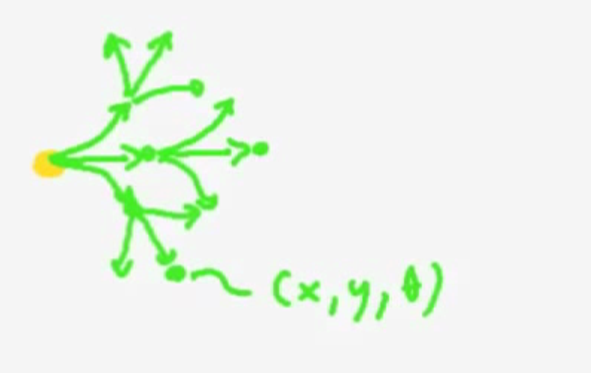
\includegraphics[scale=0.95]{../FIGURES/fig84}
\end{figure}

Therefore, the car path planning algorithm starts in the pose A the
search of the optimal path to the goal pose. It starts checking the
pose A. Then, it checks three other poses generated from the pose
A. Then, for each reached pose it has to check other three poses and
so on and so forth. So, in the first search stage the algorithm checks
one pose (pose A). In the next search stage the algorithm checks 3
poses. In the next search stage the algorithm checks 9 poses, etc.
And since the algorithm never visits a pose that was generated earlier
when the algorithm has found the optimal path, let's say, comprises
by $d$ poses, the number of checked poses rises to:

\[
N \, = \, 1 \, + \, 3  \, + \, 9 \, + \, \ldots \, + \, 3^d \, \approx \, 1.5 \, \cdot \, 3^d
\]

\begin{figure}[H]
\centering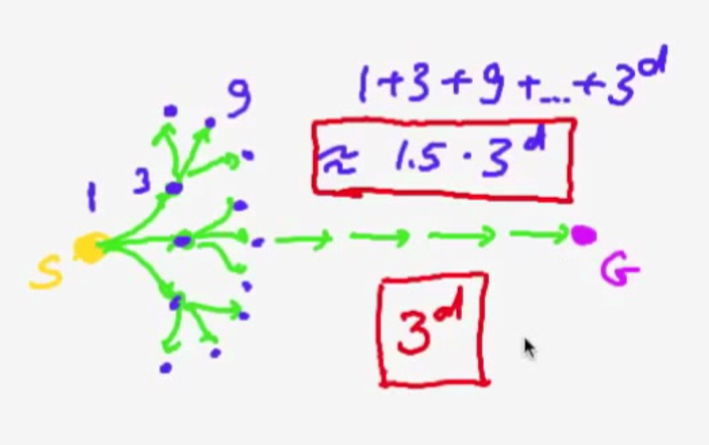
\includegraphics[scale=0.95]{../FIGURES/fig85}
\end{figure}

This enormous amount of checked poses is the problem in this algorithm.
In the A{*} algorithm (and in the Dijkstra algorithm) we have a quadratic
growth with the length of the path, $d^2$, but in this algorithm
we have an exponential growth with the length of the path, $3^d$.
This exponential growth will kill any computer. Imagine you buy a
new computer which is three times faster than your previous computer
and what you can do with that newly faster computer is to solve a
path that is just one step longer than your previous path.

The search space grows so fast that the algorithm has no chance no
matter how fast our computers are. Therefore, we need to do something
else here. One way to solve this problem is to introduce a \emph{discrete
space of possible poses.} 

Earlier in the A{*} algorithm there was a discrete raster and whenever
the algorithm had marked some nodes as visited it didn't have to add
them later on because this flag indicated that those nodes were already
in the set of optimal nodes. Now we do something similar. The algorithm
works with poses, comprises by two real coordinates of position, $x$,
and $y$, and a real coordinate of orientation, $\theta$. Therefore,
now the algorithm is going to work with a 3D raster, i.e, a 3D space
of discrete poses or discrete states. For example we could use unit
steps for the raster of the position coordinates, $x$ and $y$, and
a 10-degree step for the raster of the heading angle, $\theta$ ($\theta \, = \, 10k$,
where $k \, = \, 0, \, \ldots, \, 35$).

\begin{figure}[H]
\centering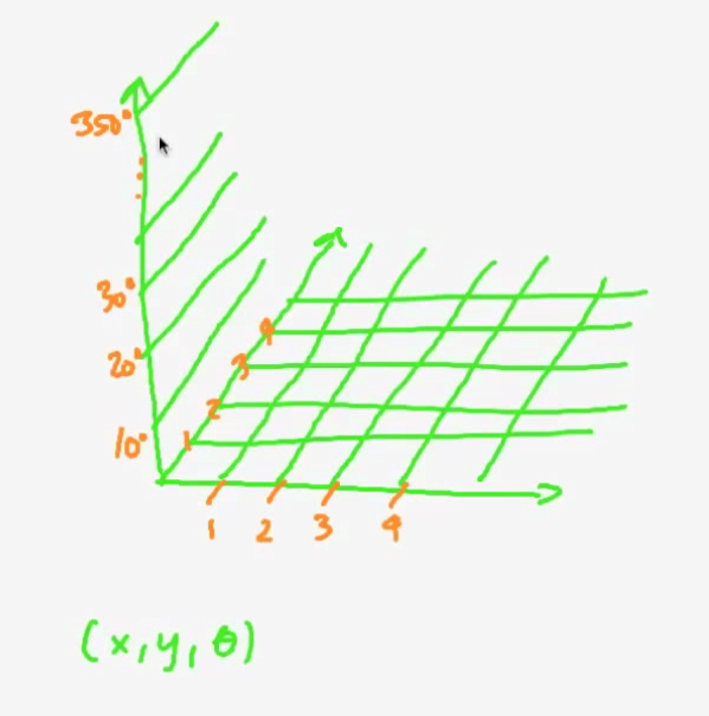
\includegraphics[scale=0.95]{../FIGURES/fig86}
\end{figure}

For example the continuous pose $\left(2.4, \, 1.2, \, 10^{\circ}\right)$
will be converted into the 3D cell (or 3D node) $\left[2, \, 1, \, 1 \right]$.
If the algorithm moves on from this pose to the pose, let's say, $\left(5.1, \, 11.9, \, 89.2^{\circ}\right)$,
the 3D cell (or 3D node) generated will be $\left[5, \, 11, \, 8 \right]$.

\begin{figure}[H]
\centering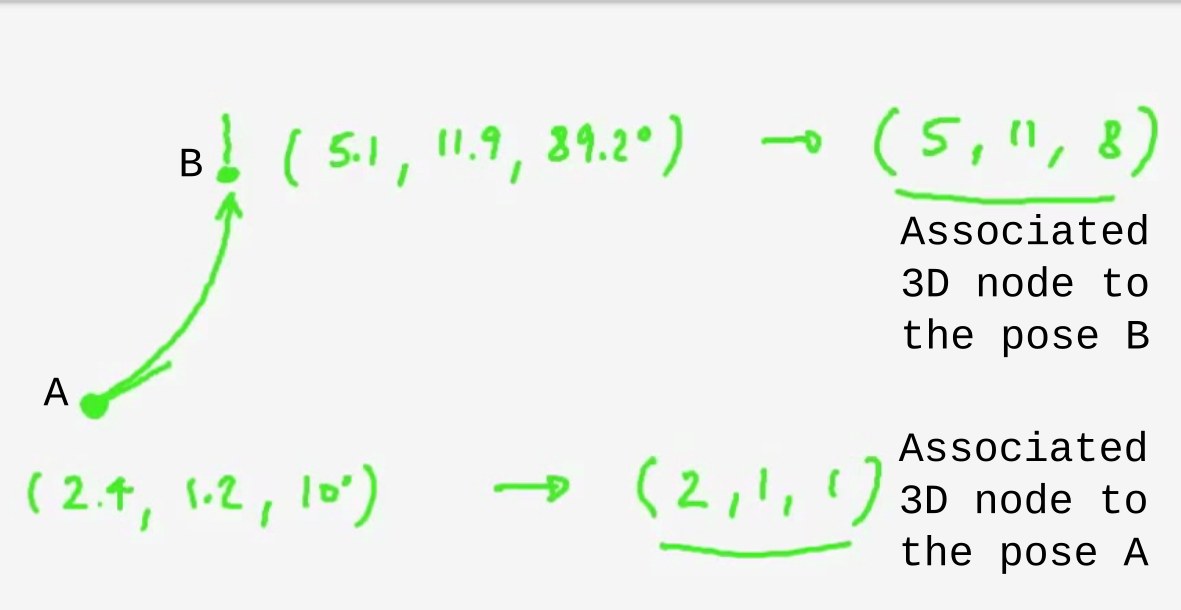
\includegraphics[scale=0.95]{../FIGURES/fig87}
\end{figure}

So, by marking those two 3D nodes as visited (node associated to the
pose A and node associated to the pose B) the algorithm prevents the
case where a new pose very similar to the pose B is generated from
another pose (pose C in next graphic). This new pose very similar
to the pose B would produce the same 3D node as the pose B, but that
3D node was marked previously as visited, so it is already included
in the path to the goal and it can't be included twice. So, because
that 3D node is not produced again that new pose, pretty similar to
the pose B, is not explored.

\begin{figure}[H]
\centering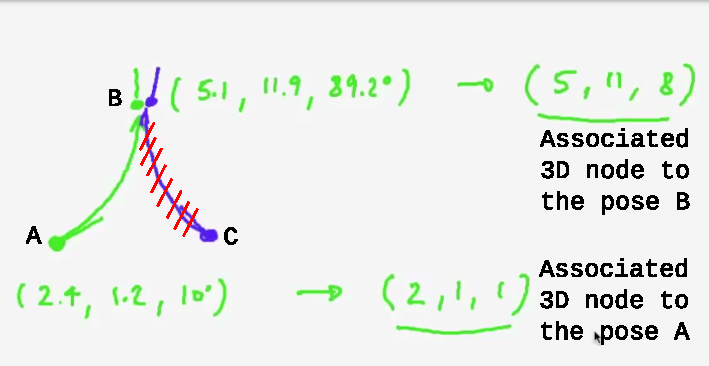
\includegraphics[scale=0.95]{../FIGURES/fig88}
\end{figure}

This behavior prevents the rapid growth of the search space. On the
other hand it has to be noted that since in this case the algorithm
doesn't explore the transition between the pose C and that pose pretty
similar to the pose B the returned path is not probably optimum anymore.
However, it works pretty well.

\begin{figure}[H]
\centering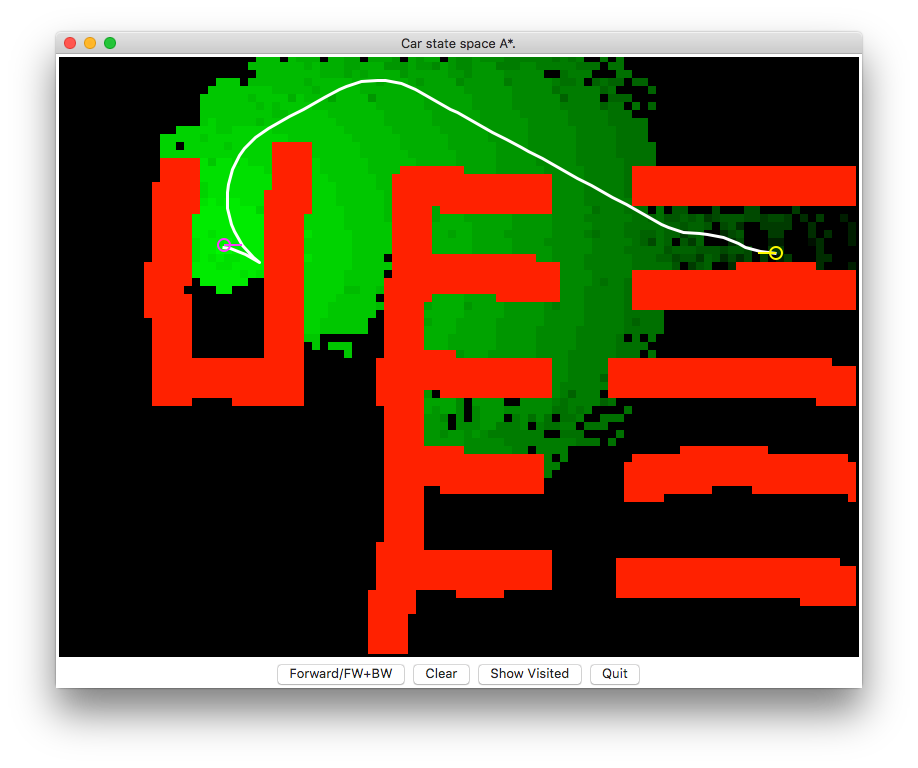
\includegraphics[scale=0.5]{../FIGURES/fig89}
\end{figure}

\end{document}
